\documentclass[10pt,a4paper]{article}

\usepackage[italian]{babel}
\usepackage{amsmath}
\usepackage{amsfonts}
\usepackage{amssymb}

\usepackage[left=1cm,right=1cm,top=1cm,bottom=2cm]{geometry}

\usepackage{txfonts}
\usepackage[T1]{fontenc}
\usepackage[utf8]{inputenc}

\usepackage{titlesec}
\setcounter{secnumdepth}{4}
\titleformat{\paragraph}{\normalfont\normalsize\bfseries}{\theparagraph}{1em}{}
\titlespacing*{\paragraph}{0pt}{3.25ex plus 1ex minus .2ex}{1.5ex plus .2ex}

\usepackage{graphicx}
\usepackage{subcaption}

\usepackage{wrapfig}

\pagenumbering{arabic}
\pagestyle{plain}

% per non farlo anadre a capo ovunque
\usepackage[none]{hyphenat}
% per togliere gli ident all'inizio dei paragrafi
\setlength{\parindent}{0pt}

\begin{document}
\subsection{Scheda enbedded}
Per questo progetto abbiamo realizzato una scheda enbedded che comprendesse l'imu, un modulo bluetooth, la batteria con il suo regolatore e un arduino.

\begin{figure}[h]
	\centering
	\vspace{-10pt}
	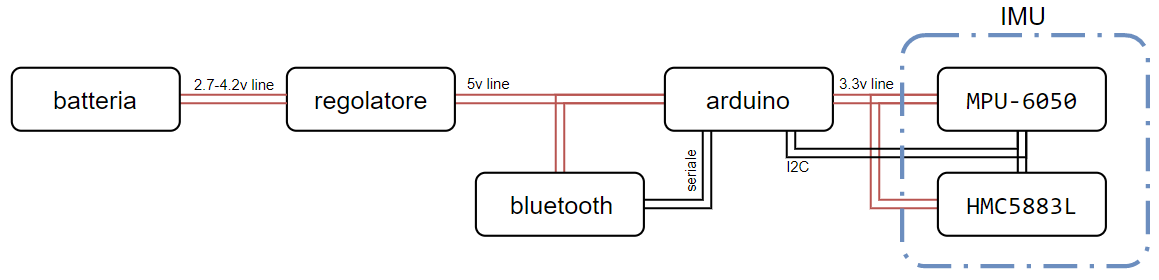
\includegraphics[width=0.80\textwidth]{scheda.png}
	\vspace{-10pt}
	\caption{Schema scheda enbedded}
	\label{fig:scheda}
\end{figure}

foto scheda

(..c'e' da dire altro?)

\subsubsection{Arduino}

\begin{wrapfigure}{r}{0.2\textwidth}
	\centering
	\vspace{-30pt}
	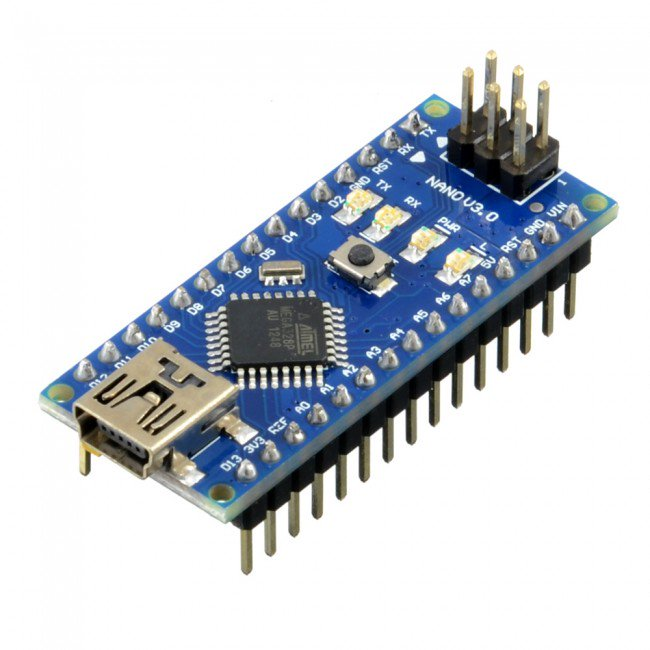
\includegraphics[width=0.2\textwidth]{arduino.jpg}
	\vspace{-30pt}
	\caption{Arduino nano}
	\label{fig:arduino_nano}
	\vspace{-30pt}
\end{wrapfigure}

Arduino \`e una piattaforma hardware open-source dotata di microcontrollore e tutto il suo ecosistema. Questo la rendono un ottima scheda per la prototipazione rapida (..da ristrutturare la frase). Nel nostro progetto abbiamo usato la scheda "Arduino nano" (fig.\ref{fig:arduino_nano}).
(..da aggiunge che e' alimentata a 5v)
La scheda si interfaccia al pc per essere programmata, tramite "Arduino IDE", e ha al suo interno un regolatore di tensione da 5V a 3.3V, utile per alimentare accelerometro e magnetometro.
\\
(..ce la metto una breve lista delle periferiche?)
\\
(.. tipo ha l'I2C, seriale, che micro e' etc..)

\vspace{10pt}

\subsubsection{Bluetooth}
\begin{wrapfigure}{r}{0.2\textwidth}
	\centering
	\vspace{-30pt}
	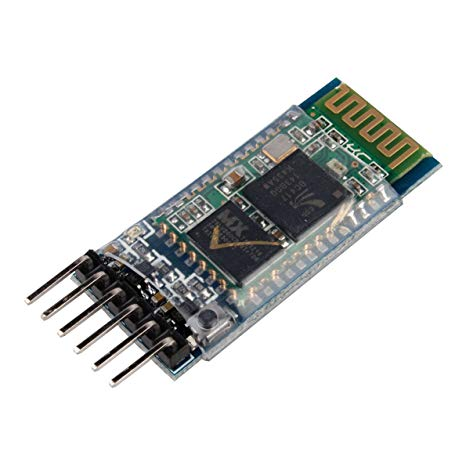
\includegraphics[width=0.2\textwidth]{HC-05.jpg}
	\vspace{-30pt}
	\caption{HC-05}
	\label{fig:HC-05}
	\vspace{-30pt}
\end{wrapfigure}
Il modulo bluetooth ulilizzato \`e "HC-05", questo modulo deve essere alimentato a 5V. Per comunicare con arduino usa la seriale (RS-232) con livello logico 3.3V, ci\`o comporta la necessit\`a di inserire un partitore sul pin rx del modulo (quindi il pin tx di arduino).
\\
(..sta cosa la mettiamo qua o da qualche altra parte?->qui->ok)

\hfill \break
\hfill \break
\hfill \break


\subsubsection{L'imu}

L'imu (inertial measurement unit) serve (..serve non va bene) a misurare le forze ad esso applicate e l'orientazione dello stesso. Questo viene solitamente fatto combinando i dati di accelerometro, magnetometro e giroscopio. In particolare l'accelerometro misura le accelerazioni, da cui in condizioni di moto inerziale si pu\`o estrarre il vettore gravit\`a sui 3 assi determinando quindi l'angolazione rispetto al suolo; Il magnetometro rileva invece il campo magnetico terrestre su 3 assi, dando cos\`i indicazione della direzione "nord"; Infine il giroscopio restituisce le accelerazioni angolari.
Per questo specifico progetto si sono utilizzati i moduli commerciali "MPU-6050" (fig.\ref{fig:MPU6050}) e "HMC5883L" (fig.\ref{fig:HMC5883L}), rispettivamente come accelerometro pi\`u giroscopio e magnetometro. 

\begin{figure}[h]
    \centering
    \begin{subfigure}[b]{0.3\textwidth}
        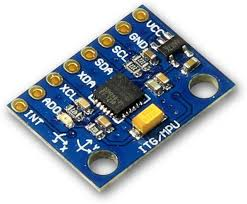
\includegraphics[height=0.75\textwidth]{MPU-6050.jpg}
        \caption{MPU-6050}
        \label{fig:MPU6050}
    \end{subfigure} 
    \begin{subfigure}[b]{0.3\textwidth}
        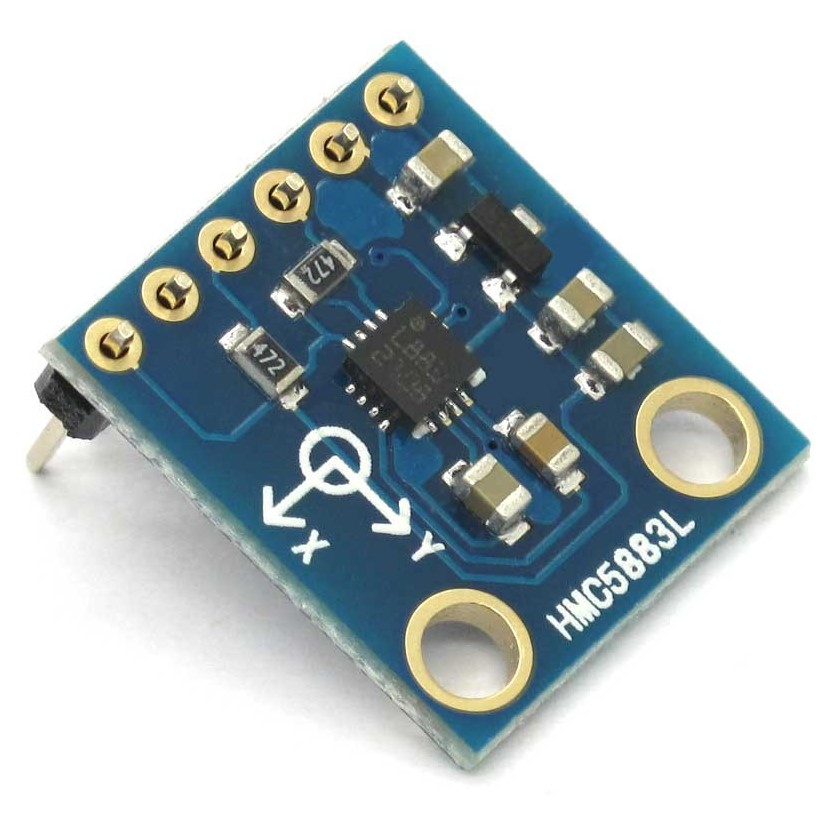
\includegraphics[height=0.75\textwidth]{HMC5883L.jpg}
        \caption{HMC5883L}
        \label{fig:HMC5883L}
    \end{subfigure}
    \caption{l'IMU utilizzata in questo progetto}
    \label{fig:imu}
\end{figure}

Questi dispositivi comunicano con arduino attraverso il protocollo I2C.




\end{document}